\chapter{Baza danych}
\section{Model danych}
Model danych w aplikacji składa się z 4 tabel znajdujących się w bazie danych oraz enuma, który trzyma klasę obiektu.\ Cechą wspólną obiektów jest posiadane przez nie pole \textbf{Id}, które służy za identyfikację danych.\ Pole to jest typu \textit{string}.\ Jak można zobaczyć na \refsource{modelu}{fig:db}

\begin{figure}[H]
    \centering
    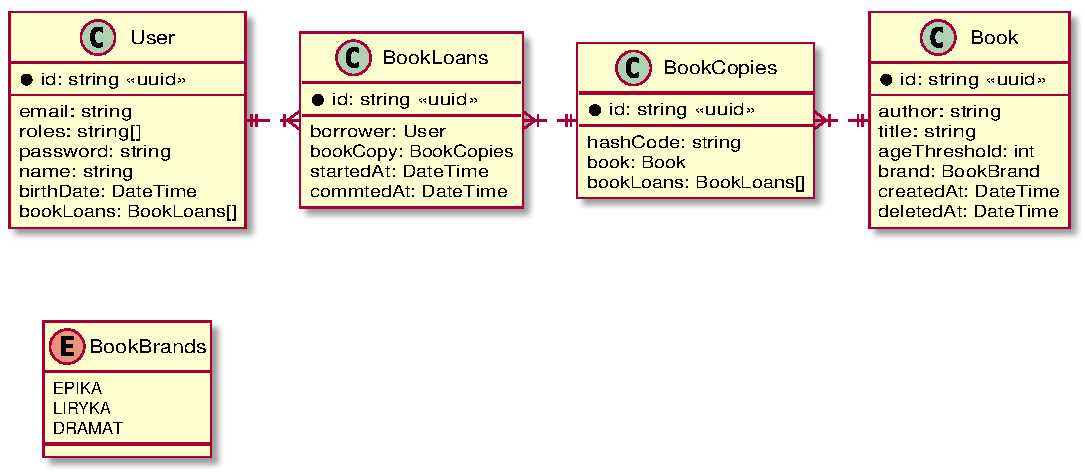
\includegraphics[width=\textwidth]{images/class}
    \captionsource{Model danych}{Opracowanie własne}
    \label{fig:db}
\end{figure}

obiekt \textbf{BookBrands}, który jest enumem, określa informacje dotyczące gatunku książki.\ Tabela \textbf{User} przetrzymuje informacje o użytkownikach, oraz łączy się z tabelą \textbf{BookLoans} relacją jeden do wielu, co oznacza, że jeden użytkownik, może wypożyczyć wiele książek.\ Tabela \textbf{BookLoans} łączy się relacją wiele do jednego z tabelą \textbf{BookCopies} co oznacza, że jeden egzemplarz książki może być wypożyczony wiele razy. Dodatkowo tabela \textbf{BookCopies} łaczy się z tabelą \textbf{Books} relacją wiele do jednego, ponieważ jedna książka może mieć wiele kopii.

\section{Replikacja bazy danych}
Replikacja bazy danych to umożliwienie automatycznego rozgłoszenia danych, przez jednostkę nadrzędną (\textit{master}) do jednostek podrzędnych (\textit{slave}). W projekcie wykorzystującym bazę danych PostgreSQL \cite{Pos2023} zastosowano replikację master-master.\ Replikacja ta pozwala na to, aby każdy serwer bazy danych był serwerem równorzędnym, co pozwala na zapisywania i odczytywanie danych z każdego serwera, dzięki czemu podczas awarii jednego mastera, drugi może przejąć jego ruch.\ Do uruchomienia takiej usługi wykorzystano oprogramowanie Bucardo \cite{Buc2023}.\ Bucardo jest to system wspomagający replikację bazy danych.\ Łączy się do wielu baz danych i umożliwia działanie na zasadzie ''\textit{Wyzwalacza}'', który propaguje dane z jednej bazy na wszystkie pozostałe.\ Oprogramowanie to trzeba zainstalować dodatkowo na serwerach baz danych, aby mógł on rozgłaszać dane, którą są dodawane, usuwane, zmieniane.\ Wykorzystanie Bucardo okazało się koniecznym krokiem, przez wzgląd na to, że PostgreSQL \cite{Pos2023}, nie posiada wbudowanej replikacji master-master.\ Dodatkowo Bucardo nie umożliwia replikacji danych znajdujących się przed jego uruchomieniem na serwerze bazodanowym.


\section{Widok tabel}
Tabele w bazie danych wyglądają tak jak na \refsource{zdjęciu}{fig:db1}.\ Dodatkowo tabela \textbf{Book}, prezentuje się jak na \refsource{zrzucie}{fig:db1}.

\begin{figure}[H]
    \centering
    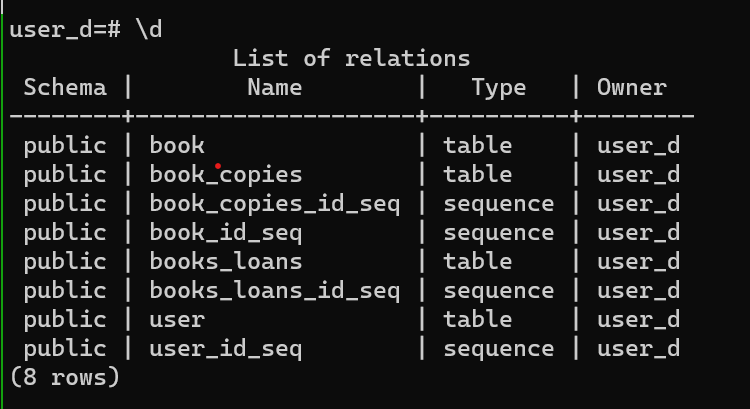
\includegraphics[width=\textwidth]{images/db1}
    \captionsource{Zrzut tabel}{Opracowanie własne}
    \label{fig:db1}
\end{figure}

\begin{figure}[H]
    \centering
    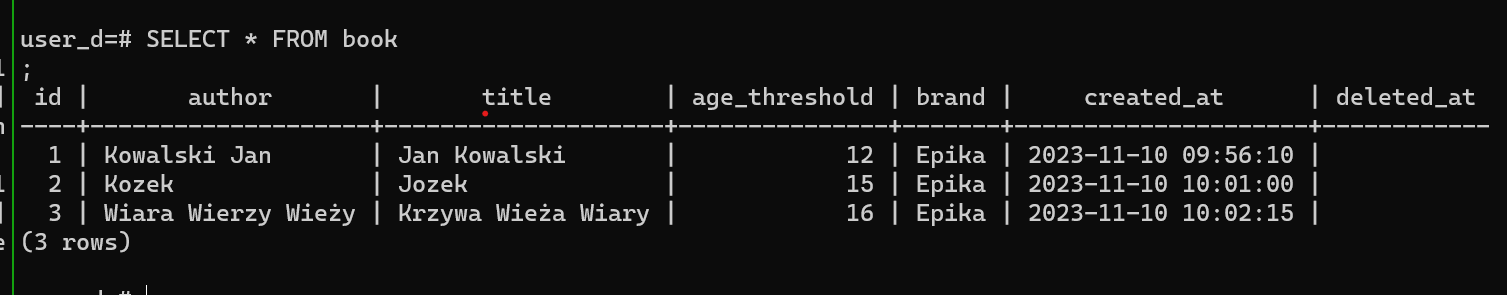
\includegraphics[width=\textwidth]{images/db2}
    \captionsource{Wyniki zapytania SELECT na tabeli book}{Opracowanie własne}
    \label{fig:db2}
\end{figure}
